\subsection{Johanneberg 7:8 – en beskrivning av fastigheten på Walleniusgatan}

% Hur tänkte de när de byggde och renoverade huset?
% Vad ville de uppnå och vilka regler och normer hade man att hålla sig till?

% Att huset är byggt så här vad betyder det för hur huset påverkas och hur huset är att bo i?

% Det är så här stort och har så här många rum, så här högt i tak o.s.v. 

Huset uppfördes 1935\cite{ritningar_urspr} och sedan kom det att dröja ända till 1988 innan den första större ombyggnationen gjordes. Då gjordes två lägenheter om till kontor, stammar byttes och vinden byggdes om till lägenheter. Både taket, burspråken på södersidan och den norra fasaden tilläggsisolerades. I samband med detta installerades också nya värme- och ventialtionssystem och alla fönster tätades med expanderskum. Den främsta skillnaden för de boende blev minskat drag och bättre luftgenomströmmning.  Med det nya venitlationssystemet byts luften helt och hållet varannan timme. Enligt Peter Särneö\cite{petersarneo} förbrukar fastigheten idag mindre energi än ett nybyggt hus.

Fastigheten 13 lägenheter och en kontorslokal på $\unit[225]{m^2}$. De utgör tillsammans $\unit[1450]{m^2}$ fördelat på sju våningar. Utöver detta finns det gemensamma utrymme, trapphus, förråd och apparatrum i den nedre källaren och Peter Särneö\cite{petersarneo} bedömmer att det totalt rör sig om ca $\unit[2000]{m^2}$. Sedan ett tag tillbaka har även en väderstation installerats i förhoppningen att den ska kunna utnyttjas för att förbättra fastighetens klimat ytterligare, se avsnitt \ref{subsec_weatertransmitter}.


% De olika gränsytornas material och uppbyggnad.
\subsubsection{Väggarna}
Ytterväggarna bestod ursprungligen av 50 cm tegel, klätt med ett centimetertjockt lager av puts på insidan, se figur \ref{fig:sodervagg}. Norrväggen, som tilläggsisolerades i samband med renoveringen 1988, har dessuotm 2 cm puts, 10 cm mineralull och ytterligare 2 cm puts utanpå tegelväggen, se figur \ref{fig:norrvagg}.\cite{kandidatarbete2010}\cite{petersarneo}

\begin{figure}[hpbt]
\centering
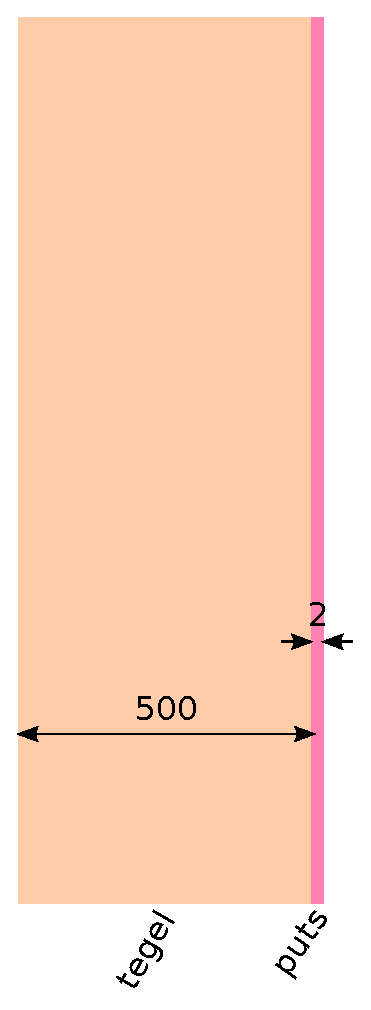
\includegraphics[width=0.6\textwidth]{images/sodervagg.eps}
\caption{\label{fig:sodervagg}{Söderväggen, utifrån och in från vänster till höger.}}
\end{figure}

\begin{figure}[hpbt]
\centering
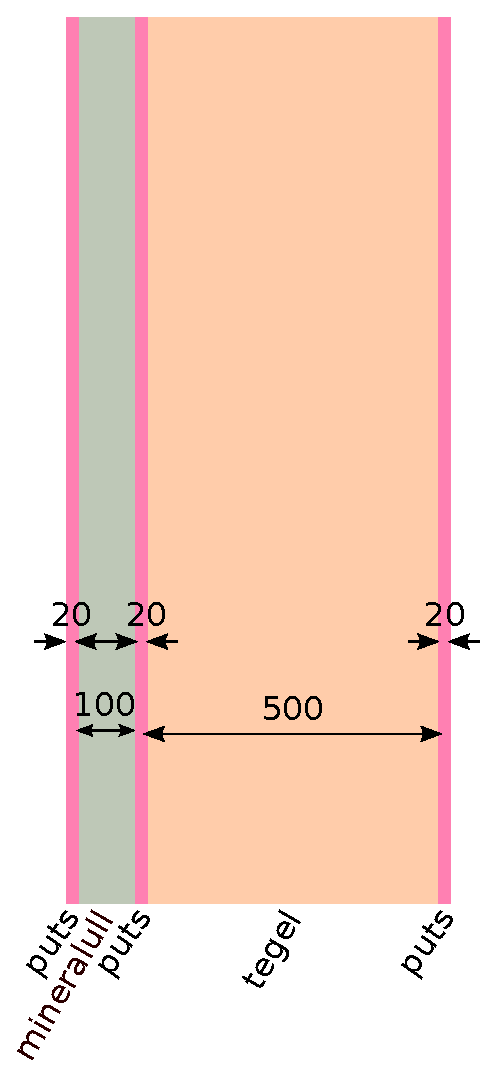
\includegraphics[width=0.6\textwidth]{images/norrvagg.eps}
\caption{\label{fig:sodervagg}{Norrväggen, utifrån och in från vänster till höger.}}
\end{figure}

På söderväggen finns ett burspråk som är kopparklätt kopparn sitter direkt på en cementbunden spånskiva och sedan en luftspalt om ca 2,5 cm. Väggen innanför består av 1,6 cm gips, 5 cm minneralull och sedan ytterligare 2,4 cm gips, se figur \ref{fig:bursprak}.\cite{kandidatarbete2010} Enligt Peter Särneö\cite{petersarneo} är det burspråket som läcker mest energi.

\begin{figure}[hpbt]
\centering
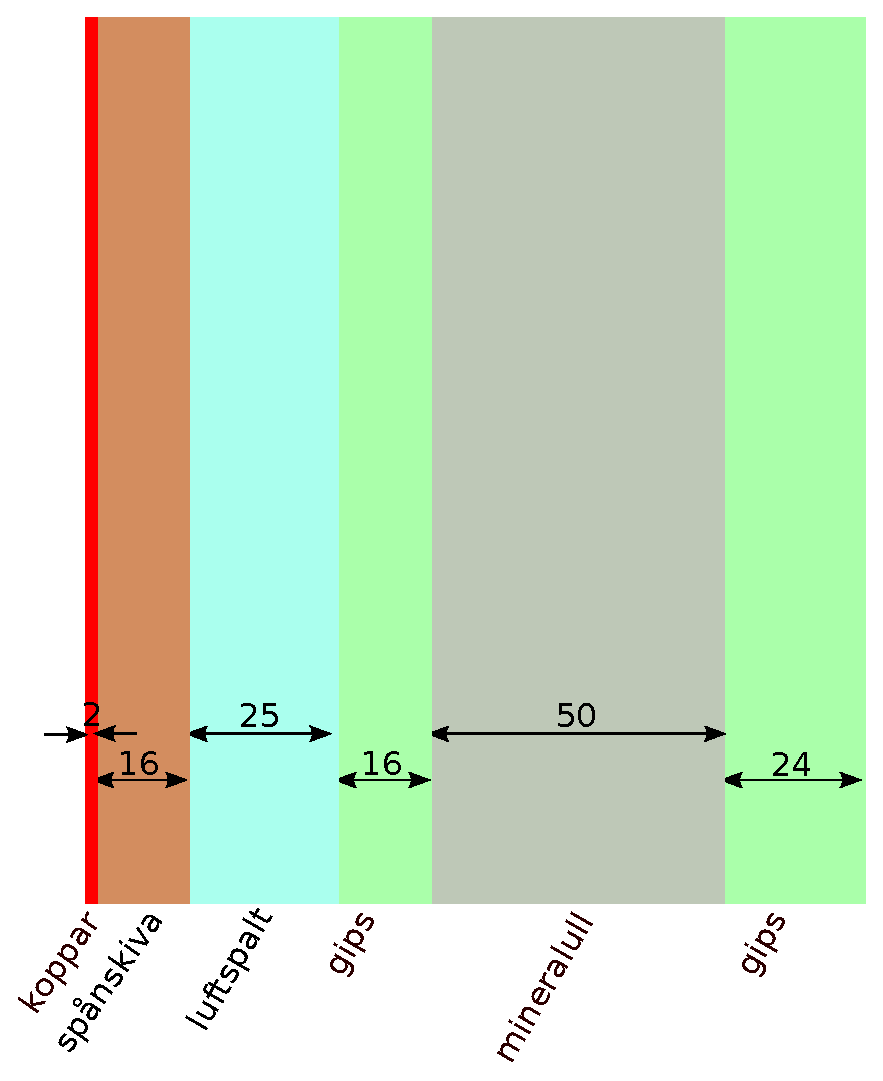
\includegraphics[width=0.6\textwidth]{images/bursprak.eps}
\caption{\label{fig:sodervagg}{Burspråket på söderväggen, utifrån och in från vänster till höger.}}
\end{figure}

\subsubsection{Taket}

\begin{figure}[hpbt]
\centering
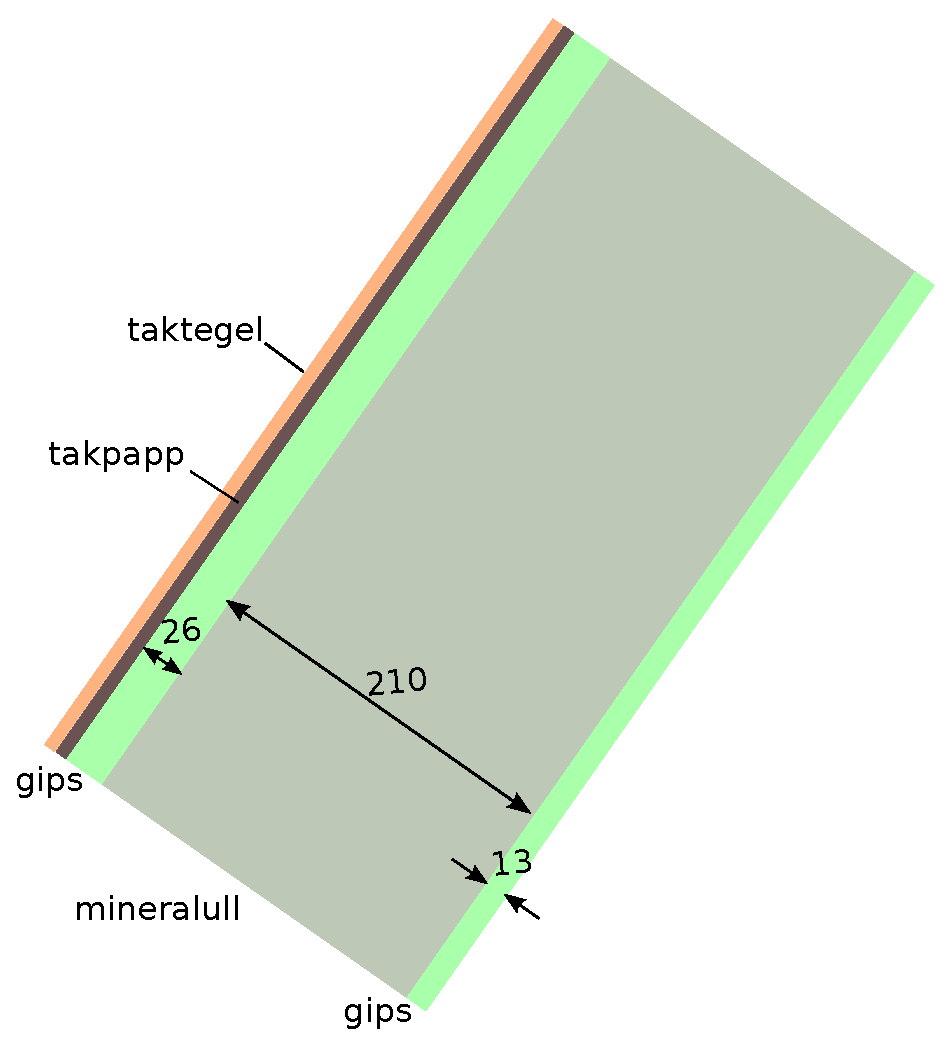
\includegraphics[width=0.6\textwidth]{images/taket.eps}
\caption{\label{fig:sodervagg}{Taket.}}
\end{figure}

\subsubsection{Grunden}

Huset är byggt på ett berg som sluttar kraftigt. I östra delen av fastigheten ligger huset direkt på berget med endast ett lager av makadam emellan\cite{petersarneo}. I västra halvan har huset en undre källare, det är där apparat- och fläktrummen finns. Där är det betydligt större avstånd ned till berget, uppskattningsvis ett par meter. % Källa?

\subsubsection{Uppvärmning och ventilation}
Idag värms huset av bergvärme. För att minska energiåtgången har ett flertal värmeväxlare installerats och värmen från all frånluft återanvänds i möjligaste mån.
% Hur fungerar regleringen? Källa?
Det är viktigt att lägenheterna är kalibrerade så att de får samma temperatur vid samma energiutflöde.


